\documentclass[]{article}
\usepackage[german]{babel}
\usepackage{graphicx}
\usepackage{tabularx}
\usepackage[backend=bibtex, natbib=true]{biblatex}
\usepackage{listings}
\usepackage{tikz}

\lstset{%
	basicstyle=\ttfamily\scriptsize,        % Code font, Examples: \footnotesize, \ttfamily
	keywordstyle=\color{blue!80!black},     % Keywords font ('*' = uppercase)
	commentstyle=\color{gray},              % Comments font
	numbers=left,                           % Line nums position
	numberstyle=\tiny,                      % Line-numbers fonts
	stepnumber=1,                           % Step between two line-numbers
	numbersep=5pt,                          % How far are line-numbers from code
	backgroundcolor=\color{gray!10!white},  % Choose background color
	frame=none,                             % A frame around the code
	tabsize=2,                              % Default tab size
	captionpos=b,                           % Caption-position = bottom
	breaklines=true,                        % Automatic line breaking?
	breakatwhitespace=false,                % Automatic breaks only at whitespace?
	showspaces=false,                       % Dont make spaces visible
	showstringspaces=false                  %
	showtabs=false,                         % Dont make tabls visible
	columns=flexible,                       % Column format
	morekeywords={},                        % Specific keywords
	stringstyle=\color{green!50!black},%
}%

\bibliography{bibliography}
%opening
%Here you can enter your names and titleof your report
\title{Weekly Reports}
\author{Luftqualität in Innenräumen - Gruppe 1}

\begin{document}

\maketitle

\begin{table}[h!]
	\centering
	\begin{tabular}{|c|c|c|}
		\hline
		{\textbf{Name}}				&		{\textbf{Matrikel Nr.}} & {\textbf{Arbeitsaufwand (h)}} \\
		\hline
		Friedrich Just				&		1326699 				&		\\
		\hline
		Stipe Knez				&		1269206 				&	\\
		\hline
		Lucas Merkert				&		1326709					&	20,00	\\
		\hline
		Achim Glaesmann				&		1309221					&		\\
		\hline
		Max-Rene Konieczka			&		1211092					&		\\
		\hline
		Can Cihan Nazlier			&		1179244					&		\\
		\hline
	\end{tabular}
	\caption{Arbeitsaufwand dieser Woche}
	\label{tab:worakload}
\end{table}



\section{Überblick}


\subsection{Friedrich Just}



\subsection{Stipe Knez}

\subsection{Lucas Merkert}
Diese Woche wurde der CCS811 Sensor zum laufen gebracht. Hierbei haben wir uns mithilfe der Informationen von Dienstag einen geeigneten Zustandsautomaten wie in Abbildung \ref{img:Zustandsautomat} überlegt und diesen dann umgesetzt. Hierbei wurde der Sensor über die Adresse 0x5A angesprochen angesprochen. Im ersten Zustand wechselt der Sensor in den BOOT Modus damit ein Software-Reset durchgeführt werden kann und die Hardware ID überprüft werden kann. Danach wechselt der Sensor wieder in den APP Modus. In das MEAS\_MODE Register wird dann der Befehl geschrieben, dass der Sensor jede Sekunde misst. Zuletzt wird noch im Status Register überprüft ob Daten bereit liegen und diese werden dann ausgelesen. Dies geschieht in einem Zyklus von einer Sekunde.

\begin{figure}[h]
	\centering
	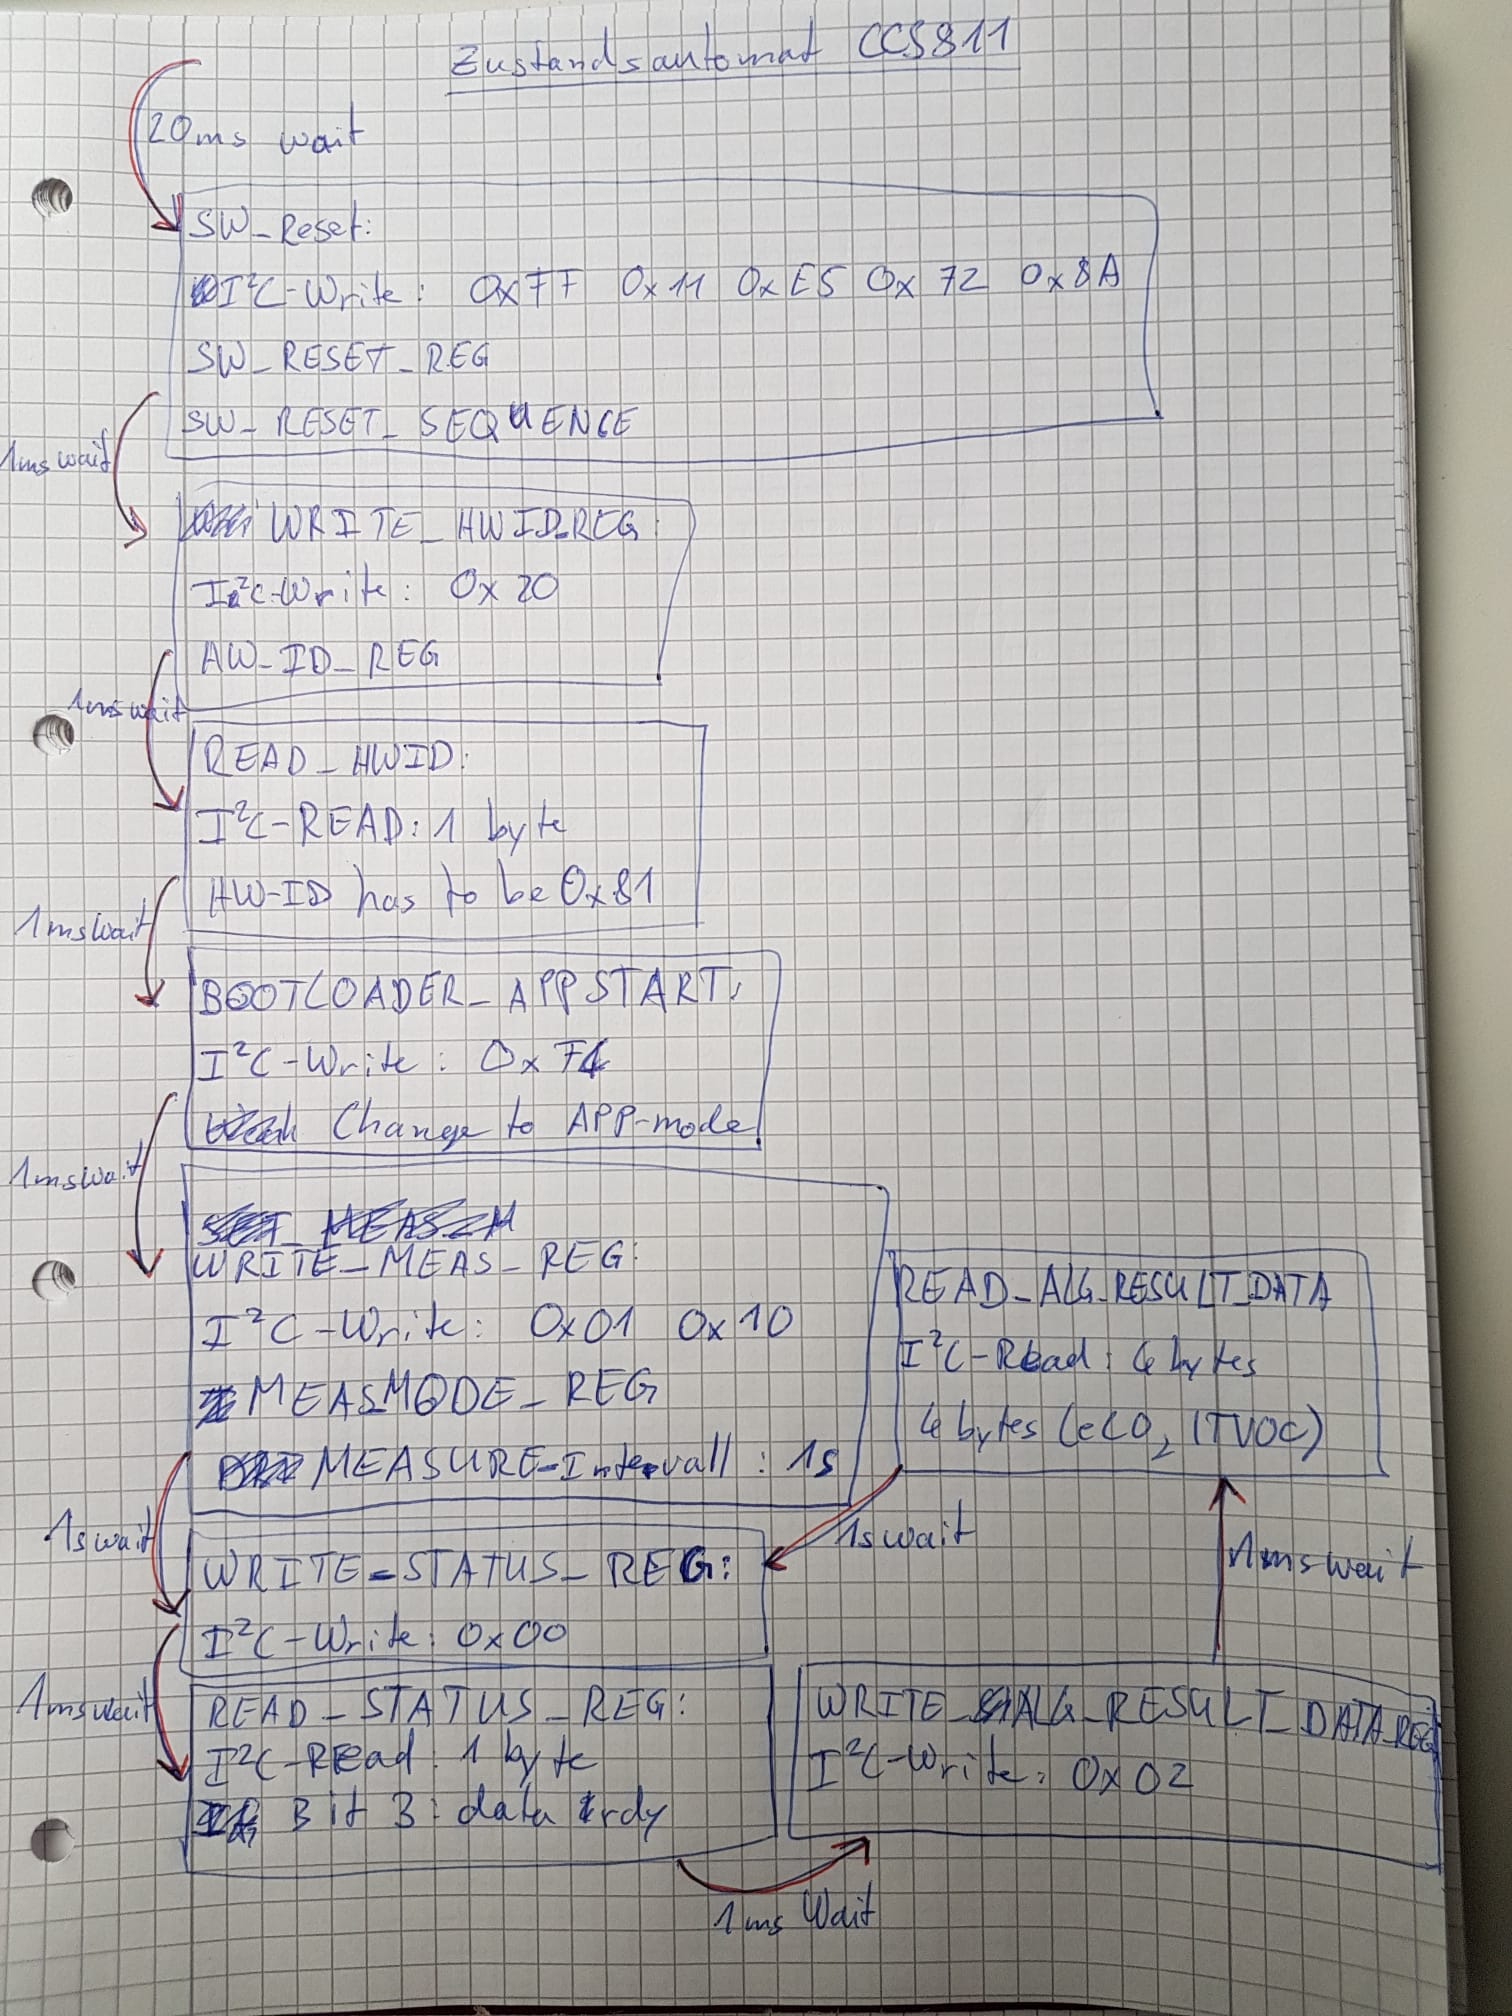
\includegraphics[scale=0.20]{images/zustandsautomat_ccs811}
	\caption{Zustandsautomat CCS811}
	\label{img:Zustandsautomat}
\end{figure}

\subsection{Achim Glaesmann}


\subsection{Max-Rene Konieczka}

\subsection{Can Cihan Nazlier}


\printbibliography
%----------------------------------------------------------------------------
% Bibliography
%----------------------------------------------------------------------------	

\end{document}
